\chapter{Astrodynamics}
\label{chap:astrodynamics}

\hl{Donald}

\section{Universe}
\label{sec:universe}

The \texttt{Universe} class is the central storage class for all celestial body and ephemeris data required by EMTG. EMTG creates a single \texttt{Universe} object for each \texttt{Journey} in the EMTG mission shortly after the EMTG options file is parsed. An emtg\_universe file is passed to the \texttt{universe} constructor and parsed using the \texttt{load\_universe\_data} method. If \texttt{SplineEphem} \ref{chap:splineephem} is being used, then a \texttt{SplineEphem\_universe} is also created and passed to the \texttt{Universe} constructor so that a spline-smoothed ephemeris may be used. The \texttt{universe} constructor also creates a \texttt{CentralBody} object that corresponds to the central body specified in the emtg\_universe file. The \texttt{universe} objects that correspond to the \texttt{Journeys} in an EMTG mission are connected together in a singly-linked list, the current \texttt{universe} has a pointer to the next \texttt{universe} in the mission to facilitate SOI transitions across \texttt{EphemerisReferenced} boundary events. The \texttt{next\_universe} pointer is accessed via the \texttt{get\_nextUniverse()} method.

An EMTG \texttt{universe} mostly contains astrodynamics data pertaining to the \texttt{CentralBody} (\ref{sec:central_body}), whose geometric center serves as the center of propagation in EMTG. The \texttt{locate\_central\_body} method computes the Cartesian state of the \texttt{CentralBody} with respect to the Sun, and returns zero, if the \texttt{CentralBody} is the Sun. A \texttt{universe} also contains a vector of \texttt{Body} objects for each of the perturbation/flyby targets available in a .emtg\_universe file. A \texttt{Frame} object is constructed using the \texttt{CentralBody} IAU Euler rotation angles (\ref{sec:frame}) and their first time derivatives $\{\alpha, \dot{\alpha}, \delta, \dot{\delta}, W, \dot{W}\}$ that are specified in a .emtg\_universe file. Gas drag on a spacecraft due to the atmosphere of the \texttt{CentralBody} can be modeled as discussed in section \ref{sec:AerodynamicDragTerm}. To facilitate this, if it is required, an \texttt{atmosphere} object is constructed for each \texttt{universe} object that requires one. This is done shortly after the \texttt{universes} are assembled in the main \texttt{EMTG\_v9.cpp} execution method.

The \texttt{universe} also contains some of the scaling information used by EMTG when it assembles the NLP problem passed to the NLP solver. The \texttt{continuity\_constraint\_scale\_factors} container contains multiplicative scaling factors that are applied to all trajectory defect constraints that appear in EMTG's trajectory transcriptions. Position defects are multiplied by $1/LU$, where $LU$ is specified by the user in the emtg\_universe file. A time scaling unit $TU$ is computed using the \texttt{CentralBody} $\mu$ and the provided $LU$. Velocity defects are multiplied by $TU/LU$. Mass defects are multiplied by $1/MU$ where $MU$ is the upper bound on the spacecraft's initial mass. Finally, time/epoch defects are multiplied by $1/TU$.


\section{Body}
\label{sec:body}

\hl{Donald}

Each \texttt{body} class owns a \texttt{frame} object and a \texttt{bplane} object.

\section{CentralBody}
\label{sec:central_body}



\section{Frame}
\label{sec:frame}

The \texttt{Frame} class handles transformations between EMTG's available reference frames. EMTG supports the following reference frames:

\begin{itemize}
	\item \textbf{\texttt{ICRF}}: A frame aligned with the International Celestial Reference Frame (ICRF) as defined in the \ac{IAU} Cartographic Coordinates and Rotational Elements document \cite{IAU_cartographic_coordinates_2018} and in \ac{SPICE} \cite{SPICE}. All of EMTG's internal calculations are performed in ICRF, so if the user specifies a state in some other frame, then the \texttt{frame} class has to transform it.
	
	\item \textbf{\texttt{J2000\_BCI (J2000 body-centered inertial)}}: A frame defined by the first two Euler rotations ($\alpha$ and $\delta$) in the \ac{IAU} Cartographic Coordinates and Rotational Elements document \cite{IAU_cartographic_coordinates_2018}, evaluated at January 1st, 2000 (J2000). This frame uses only the constant terms of the rotation, since the time-dependent terms are expressed as time since the J2000 epoch.
	
	\item \textbf{\texttt{J2000\_BCF (J2000 body-centered fixed)}}: A frame defined by a third Euler rotation beyond \texttt{J2000\_BCI} - a rotation about the \textit{z} axis by $W$ as defined in the \ac{IAU} Cartographic Coordinates and Rotational Elements document \cite{IAU_cartographic_coordinates_2018}. The first two rotations are evaluated at the J2000 epoch, but the $W$ rotation is evaluated at the epoch of the state being rotated. EMTGv9 only supports the linear component of the rotation, \textit{i.e} $W = W_0 + \dot{W}$. This was judged sufficient for EMTG's intended use cases. EMTG's \texttt{J2000\_BCF} is still an inertial frame; the time derivatives of the unit vectors of the \texttt{J2000\_BCF} frame are all zero. In other words, the position and velocity are rotated according to the IAU angles, but the velocity transformation does not include the $\mathbf{\omega} \times \mathbf{r}$ term. This is deliberate and is a definition that is often used for designing planetary probe trajectories. \hl{Kyle, Noble}
	
	\item \textbf{\texttt{TrueOfDate\_BCI (true-of-date body-centered inertial)}}: A frame identical to \texttt{J2000\_BCI} except that all three Euler rotations are evaluated at the epoch of the state being rotated.
	
	\item \textbf{\texttt{TrueOfDate\_BCF (true-of-date body-centered fixed)}}: A frame identical to \texttt{J2000\_BCF} except that all three Euler rotations are evaluated at the epoch of the state being rotated.
	
	\item \textbf{\texttt{PrincipleAxes}}: \hl{Noble}. Not yet fully implemented.
	
	\item \textbf{\texttt{Topocentric}}: \hl{Noble}. Not yet fully implemented.

	\item \textbf{\texttt{Polar}}: \hl{Noble}. Not yet fully implemented.
	
	\item \textbf{\texttt{J2000\_BCR (J2000 body-centered rotating)}}: A frame identical to \texttt{J2000\_BCF} except that the velocity vector is with respect to the rotating BCF frame. In other words, the $\mathbf{\omega} \times \mathbf{r}$ term is included, unlike in the \texttt{J2000\_BCF} frame. Not yet implemented.
	
	\item \textbf{\texttt{TrueOfDate\_BCR (true-of-date body-centered rotating)}}: A frame identical to \texttt{J2000\_BCR} except that all three Euler rotations are evaluated at the epoch of the state being rotated. Not yet implemented.
	
	\item \textbf{RIC (radial-intrack-crosstrack)}: A frame defined by the position and velocity vectors of the central body relative to some other reference body. For example, OSIRIS-REx uses a RIC frame where the \texttt{x} axis is the vector from the Sun to Bennu $\mathbf{r}$, the \texttt{z} axis is the angular momentum vector of Bennu about the sun $\mathbf{h} = \mathbf{r} \times \mathbf{v}$, and the \texttt{y} axis completes the right-handed set, $\mathbf{h} \times \mathbf{v}$. (not yet implemented)
	
	\item \textbf{SAM (sun-angular momentum, also called sun-north)}: The $x$ axis points from the central body to a reference body (\textit{i.e.} the Sun). The $y$ axis is the cross product of the \texttt{J2000BCI} spin pole and the $x$ axis. The $z$ axis complete the right-handed set.
	
	\item \textbf{Object-Referenced}: The $x$ axis points from the central body to the reference body. The $y$ axis is the velocity vector of the reference body relative to the central body. The $z$ axis completes the right-handed set and is the angular momentum vector of the reference body with respect to the central body. When this frame is used with a free point boundary condition, the first and second entries in the journey's destination list define the reference body for the departure and arrival event, respectively.
\end{itemize}

At construction, the owning object passes in the three Euler rotation angles and their first-order derivatives ($\alpha_0, \dot{\alpha}, \delta_0, \dot{\delta}, W, \dot{W}$). The \texttt{initialize\_J2000()} method is called by the constructor and creates the rotation matrices between \texttt{ICRF} and \texttt{J2000\_BCI}. These rotations are immediately available. The time-dependent transformations not evaluated immediately because the epoch of interest is not yet known. Instead, they are evaluated when the owning object, or another method of the \texttt{frame} itself, calls the \texttt{construct\_rotation\_matrices()} method. The rotations can be constructed with or without derivative information, as needed.

The owning object may then perform the transformation either by calling \textit{get\_R()} and \texttt{get\_dRdt} and performing the transformation outside the frame class, or more safely, by calling the \texttt{rotate\_frame\_to\_frame()} method. The \texttt{rotate\_frame\_to\_frame()} method performs the transformation and returns both the transformed state and its derivatives.

The \hl{\texttt{rotate\_frame\_to\_frame()} method will be the only safe way to transform to and from \texttt{Topocentric}, \texttt{Polar}, \texttt{J2000\_BCR}, and \texttt{TrueOfDate\_BCR} once they are fully implemented. We plan to force EMTG to use \texttt{rotate\_frame\_to\_frame()} everywhere, just to make sure.}

\section{StateRepresentation}
\label{sec:StateRepresentation}
The \texttt{StateRepresentation} set of classes handle the transformation between state representations. EMTG's default state representation is Cartesian. However there are times in various parts of the program where the user might specify state in another representation. This most frequently happens in \texttt{ParallelShootingStep} and \texttt{FreePointBoundary} but could be used in other places as well.

\texttt{StateRepresentationBase} is an abstract base class for state representation classes. A new derived class is written for every new state representation. These classes handle the transformation from Cartesian to the new state representation and back, and also compute the partial derivatives. It is up to the host class to put these partial derivatives into the Jacobian - \texttt{StateRepresentationBase} and its children just puts the math all in one place.

EMTG currently implements the following state representations, each of which has its own derived class:
\begin{itemize}
	\item Cartesian
	\item SphericalAZFPA
	\item SphericalRADEC
	\item Classical Orbit Elements (COE)
	\item B-plane coordinates $\left\{v_\infty, RHA, DHA, b_{radius}, b_{theta}, TA\right\}$. A full math spec is available in the ``bplane\_math.pdf'' file in the EMTG repository. Note that the b-plane reference vector for \texttt{IncomingBplaneRepresentation} is the current reference frame\'s $\hat z$ vector. It is not possible to make the reference vector depend on the state as that would result in a circular definition of the Cartesian state as a function of the b-plane coordinates.
\end{itemize}

\section{B-plane}
\label{sec:bplane}

\hl{Donald}

\section{AccelerationModel}
\label{sec:acceleration_model}

The \texttt{AccelerationModel} abstract base class establishes the interface between any derived acceleration models and EMTG's equations of motion classes (\ref{sec:Equations of Motion}) as well as any other entities that may have a need to directly it (MGALT with perturbations). The methods \texttt{AccelerationModel::setEpoch} and \texttt{AccelerationModel::setEpochJD} are used to set the current epoch (in seconds past the J2000 epoch and the Julian date in days respectively) to be used by any time-dependent acceleration terms (e.g. body rotational states, ephemeris-based gravity calculations, atmospheric drag). The \texttt{AccelerationModel::computeAcceleration} method takes a state vector and a boolean flag as its two inputs. The bool flag specifies whether the \texttt{AccelerationModel} should perform derivative computation. This method computes the instantaneous acceleration and stores the resultant \texttt{acceleration} vector. An overloaded for \texttt{computeAcceleration} can also be defined that accepts an input control vector should the \texttt{AccelerationModel} require a control term. The current acceleration vector can be extracted from the \texttt{AccelerationModel} using \texttt{AccelerationModel::getAcceleration}. The \texttt{AccelerationModel::populateInstrumentationFile} method must be implemented and should write acceleration data to the input \texttt{ofstream} for the input epoch (this method is also overloaded with a version that accepts a control vector as an input). 

\subsection{SpacecraftAccelerationModel}
\label{sec:spacecraft_acceleration_model}

The \texttt{SpacecraftAccelerationModel} class implements a Cartesian acceleration model for spacecraft motion with respect to the center of a gravitating body. A \texttt{SpacecraftAccelerationModel} can model the perturbative effects of $n$ third body gravity sources, spherical body solar radiation pressure, central body oblateness (J2) and gas drag assuming an exponential atmosphere model.

\begin{figure}[h!]
    \centering
    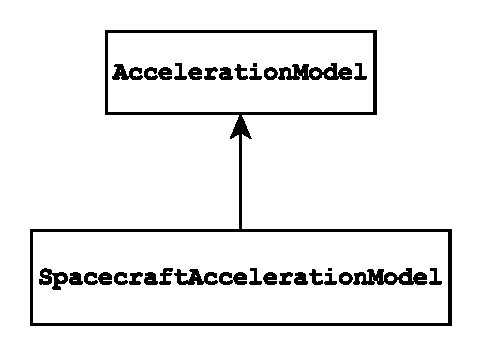
\includegraphics[width=0.3\linewidth]{./astrodynamics/AccelerationModel_inheritance.pdf}
    \caption{\label{fig:AccelerationModel_inheritance} AccelerationModel inheritance diagram.}
\end{figure} 

A \texttt{SpacecraftAccelerationModel} constructor requires pointers to a \texttt{MissionOptions} object, a \texttt{JourneyOptions} object, a \texttt{Universe} object, a vector of decision variable descriptions and a \texttt{Spacecraft} object. The input parameter \texttt{num\_STM\_size\_in} specifies the row and column dimensions the state propagation matrix that the acceleration model will compute. The boolean parameter \texttt{needCentralBody} indicates whether or not central body gravity should be included in the total acceleration calculation. This is useful for using a \texttt{SpacecraftAccelerationModel} to compute perturbations only (i.e. for an MGALT phase that models perturbation impulses, and accounts for two-body motion with respect to the central gravitating body using a \texttt{KeplerPropagator}).

On construction, the method \texttt{SpacecraftAccelerationModel::constructorInitialize} sizes various internal containers, tests if the acceleration is being computed in a heliocentric frame and then constructs whatever \texttt{SpacecraftAccelerationModelTerms} were requested by the user (via the \texttt{JourneyOptions} object pointer). During the construction of the individual \texttt{SpacecraftAccelerationModelTerms} the \texttt{needCentralBody} flag to determine if a \texttt{CentralBodyGravityTerm} is required. Calls to the \texttt{SpacecraftAccelerationModel} are categorized as heliocentric/non-heliocentric for the purposes of computing the distance from the sun for solar electric power calculations (non-heliocentric trajectories require an extra vector addition step and an associated ephemeris look-up to compute the sun-spacecraft distance).

The primary public method of the \texttt{SpacecraftAccelerationModel} is \texttt{SpacecraftAccelerationModel::computeAcceleration}, which computes and stores the acceleration experienced by the spacecraft. The inputs to this method are the spacecraft state vector, two flags indicating whether or not partial derivatives of the acceleration model should be computed and a control vector $\mathbf{u}$ (if the control overload is being called). Prior to calling this method, it is important to set the current epoch using \texttt{AccelerationModel::setEpoch} or \texttt{AccelerationModel::setEpochJD}. The majority of the public methods in \texttt{SpacecraftAccelerationModel} are get methods for extracting acceleration information from the model. These include \texttt{SpacecraftAccelerationModel::getAccelerationVec} (returns a vector of the total acceleration experienced by the spacecraft in the central body ICRF frame), \texttt{SpacecraftAccelerationModel::getGravityAccelerationVec} (returns a vector of the total gravitational acceleration on the spacecraft in the central body ICRF frame), \texttt{SpacecraftAccelerationModel::getGravityAccelSources} (returns a vector of 3-tuples, where each tuple contains a body name, body mu, and the acceleration of the spacecraft due to the body), \texttt{SpacecraftAccelerationModel::getSRPAccelerationVec} (returns the acceleration vector due to solar radiation pressure), \texttt{SpacecraftAccelerationModel::getThrustAccelerationVec} (returns the acceleration vector due to the spacecraft's thruster), \texttt{SpacecraftAccelerationModel::getThrusterMaxMassFlowRate} (returns the mass flow rate of the thruster), \texttt{SpacecraftAccelerationModel::getControlNorm} (returns the norm of the control parameters $u_x,~u_y,~u_z$), \texttt{SpacecraftAccelerationModel::getDutyCycle} (returns the duty cycle of the propulsion system), \texttt{SpacecraftAccelerationModel::getfx} (returns the state propagation matrix), \texttt{SpacecraftAccelerationModel::getSTMsize} (returns the row/column dimension of the state transition matrix), and \texttt{SpacecraftAccelerationModel::getCB2SC} (returns the distance from the central body to the spacecraft).

The \texttt{SpacecraftAccelerationModel::populateInstrumentationFile} method includes an overload with control and generates acceleration data for the current epoch and spacecraft state vector and writes it to the input \texttt{std::ofstream}. To do so, this method first writes the current JD epoch, the spacecraft state vector (including mass) and the total acceleration vector. Then, the method calls \texttt{SpacecraftAccelerationModelTerms::populateInstrumentationFile} for each term included in the acceleration calculation.

The private method \texttt{SpacecraftAccelerationModel::initializeAndComputeGeometry} zeros out the acceleration vector and the state propagation matrix (but sets the $\frac{\partial \mathbf{v}}{\partial \mathbf{v}}$ submatrix equal to $\mathbb{I}_{3\times3}$) and calls \texttt{SpacecraftAccelerationModel::computeScCbSunTriangle}. This method computes the position/velocity of the spacecraft w.r.t. the sun as well as the following partial derivative information:

\begin{align}
    &\frac{\partial \mathbf{r}_{\odot}}{\partial t} \label{eq:dr_sundepoch} \\
    &\frac{\partial \mathbf{r}_{\odot}}{\partial \Delta t_{\text{p}}} \label{eq:dr_sundflighttime}
\end{align},

\noindent where $\Delta t_{\text{p}}$ is the current phase flight time. If the trajectory is heliocentric, then Eq. (\ref{eq:dr_sundepoch}) and (\ref{eq:dr_sundflighttime}) are both zero.


\section{SpacecraftAccelerationModelTerm}
\label{sec:SpacecraftAccelerationModelTerm}

This is the abstract base class for the individual acceleration term classes in the \texttt{SpacecraftAccelerationModel}. Every \texttt{SpacecraftAccelerationModel} owns a \texttt{boost::ptr\_vector} of \texttt{SpacecraftAccelerationModelTerm} objects that are individually evaluated and polled for their contribution to the total acceleration acting on the spacecraft. The \texttt{SpacecraftAccelerationModelTerm} requires that each of its child classes define the following methods: \texttt{computeAccelerationTerm} (and its partial derivative overload), which evaluates the Cartesian acceleration contribution of the term, and \texttt{populateInstrumentationFile}, which writes acceleration data to the specified acceleration output file. The public accessor \texttt{getTermAcceleration} returns the computed acceleration contribution of the term. Each \texttt{SpacecraftAccelerationTerm} owns a member variable \texttt{SpacecraftAccelerationTerm::term\_acceleration}, which stores the acceleration contribution of the term and \texttt{SpacecraftAccelerationTerm::acceleration\_model}, which is a pointer to the \texttt{SpacecraftAccelerationModel} that owns the term object. Additional \texttt{SpacecraftAccelerationTerms} may be added to the \texttt{SpacecraftAccelerationModel} by creating them in the latter's constructor and adding their evaluation to \texttt{SpacecraftAccelerationModel::computeAcceleration}. The derived child classes that are currently implemented are described in the following subsections.

\subsection{GravityTerm}
\label{sec:GravityTerm}
\texttt{GravityTerm} contains the equations of motion that account for the acceleration due to the gravity of a point mass \texttt{Body} object on the spacecraft as well as on the \texttt{CentralBody} (center of integration). The \texttt{GravityTerm} constructor takes a pointer to its parent \texttt{SpacecraftAccelerationModel} and a pointer to the \texttt{Body} object whose gravity the class is modeling as input parameters.
The \texttt{computeAccelerationTerm} override calls the primary physics method \texttt{computePointMassGravityAcceleration} and then, if necessary, \texttt{computePointMassGravityDerivatives}. \\

The \texttt{computePointMassGravityAcceleration} method performs two main functions: 1) compute the position/velocity vectors between the \texttt{CentralBody}, the spacecraft and the gravitating point mass \texttt{Body} via a call to \texttt{computeScBodyCBtriangle} and 2) compute the acceleration on the spacecraft due to the gravitating \texttt{Body}. If the \texttt{GravityTerm} \texttt{Body} is the Sun, then the call to \texttt{computeScBodyCBtriangle} is skipped (to forgo an expensive ephemeris lookup call) as the \texttt{SpacecraftAccelerationBody::computeScCbSunTriangle} method has already been executed and has stored the position/velocity of the Sun w.r.t. the spacecraft and the \texttt{CentralBody}. Both the direct and indirect contributions of the gravity of the \texttt{Body} on the spacecraft are computed. The resultant point-mass gravity acceleration due to $i$ \texttt{Body} objects is computed in \texttt{SpacecraftAccelerationModel::computeAcceleration}:

\begin{equation}
\ddot{\mathbf{r}} = - \sum_{\text{i}} G~m_{\text{i}} \left( \frac{\mathbf{r} - \mathbf{r}_{\text{i}}}{\|\mathbf{r} - \mathbf{r}_{\text{i}}\|^3} + \frac{\mathbf{r}_{\text{i}}}{r_{\text{i}}^3} \right) \label{eq:EOM_point_mass_gravity} 
\end{equation}

\subsubsection{CentralBodyGravityTerm}
\label{sec:CentralBodyGravityTerm}

The \texttt{CentralBodyGravityTerm} class is derived from \texttt{GravityTerm} and is used to compute the acceleration of the (massless) spacecraft due to the gravity of the \texttt{CentralBody} whose geometric center coincides with the center of integration:

\begin{equation}
\ddot{\mathbf{r}} = -\frac{G \left(\cancelto{0}{m} + m_{\text{cb}}\right)}{r^2}\frac{\mathbf{r}}{r} \label{eq:EOM_central_body_gravity}
\end{equation}

The \texttt{CentralBodyGravityTerm} overrides the indirect gravitational effect of point mass gravity in \texttt{GravityTerm::computeFrameDragAcceleration} and sets that term equal to zero (since the center of integration is the center of the \texttt{CentralBody}, the \texttt{CenterBody} does not have a gravitational influence on itself, i.e. it has no trajectory w.r.t. the center of integration). The \texttt{GravityTerm::computePointMassGravityTimeDerivatives} method is similarly overrided and does nothing as the \texttt{CentralBody} gravity acceleration has no explicit time partials. \\

The \texttt{CentralBodyGravity} object also computes the acceleration on the spacecraft due to any \texttt{SphericalHarmonicTerms} that it owns in the \texttt{gravitational\_harmonic\_terms} \texttt{boost::ptr\_vector} container. At this time, only the J2 harmonic gravity term has been implemented, so the aforementioned container contains, at most, one \texttt{SphericalHarmonicTerm}.

\subsection{SphericalHarmonicTerm}
\label{sec:SphericalHarmonicTerm}
The \texttt{SphericalHarmonicTerm} class was designed to accommodate a spherical harmonic gravity model of arbitrary degree and order. Currently, only an oblateness model (J2) has been implemented. The \texttt{SphericalHarmonicTerm} constructor takes a pointer to the parent \texttt{SpacecraftAccelerationModel}, a pointer to the \texttt{Body} whose harmonic gravity this class is modeling, and a pointer to its parent/owner \texttt{CentralBodyGravityTerm}.

The \texttt{computeAccelerationTerm} method first extracts the position of the spacecraft w.r.t. the \texttt{CentralBody} by polling the \texttt{CentralBody} pointer. Next, it performs the following three actions: 1) rotate the spacecraft position into the true of date BCF frame 2) compute the acceleration due to the \texttt{CentralBody} oblateness 3) add the oblateness acceleration to the parent \texttt{CentralBody} \texttt{term\_acceleration} variable. The \texttt{computeAccelerationTerm(bool)} overload computes the acceleration due to \texttt{CentralBody} oblateness and its partial derivatives.

\begin{equation}
\label{eq:aBCFtoICRF}
\ddot{\mathbf{r}}_{J_2} = \ddot{\mathbf{r}}_{J_{2_{ICRF}}} = M^{ICRF}_{BCF}\ddot{\mathbf{r}}_{J_{2_{BCF}}}
\end{equation}

\begin{equation}
\ddot{\mathbf{r}}_{J_{2_{BCF}}} = \frac{3J_2 \mu R^2}{2r^5_{\text{BCF}}} \begin{bmatrix} 1 - 5\frac{x_{\text{BCF}}z^2_{\text{BCF}}}{r^2_{\text{BCF}}} \\ 1 - 5\frac{y_{\text{BCF}}z^2_{\text{BCF}}}{r^2_{\text{BCF}}} \\ 3 - 5\frac{z^3_{\text{BCF}}}{r^2_{\text{BCF}}} \end{bmatrix}
\end{equation}

\subsection{SolarRadiationPressureTerm}
\label{sec:SolarRadiationPressureTerm}

The \texttt{SolarRadiationPressureTerm} models spherical/cannonball solar radiation pressure. This term's constructor takes a pointer to its parent \texttt{SpacecraftAccelerationModel} as its only input parameter uses that pointer to extract the following parameters from the \texttt{MissionOptions} object: the spacecraft coefficient of reflectivity (SRP scale factor) $C_r$, the wetted surface area $A_s$, the illumination percentage $K$, solar irradiance $\phi$ at 1 AU (in $W/m^2$), and the speed of light in a vacuum $c$. The constructor also computes and stores the SRP coefficient:

\begin{equation}
C_{\text{SRP}} = \frac{C_r A_{s} K \phi}{c} \label{eq:SRP_coeff}
\end{equation}

The \texttt{computeAccelerationTerm} method calculates the instantaneous acceleration due to SRP, which is directed along the Sun-spacecraft line:

\begin{equation}
\ddot{\mathbf{r}} = C_{\text{SRP}}\frac{1}{m ~ r_{s/\odot}^2}\frac{\mathbf{r}_{s/\odot}}{r_{s/\odot}} \label{eq:EOM_SRP}
\end{equation}

\subsection{ThrustTerm}
\label{sec:ThrustTerm}

The \texttt{ThrustTerm} constructor takes a parent \texttt{SpacecraftAccelerationModel} pointer as its sole input in order to grant the class access to the \texttt{Spacecraft} (\ref{sec:spacecraft}) object to compute power system parameters, and the electric propulsion system performance parameters.

The \texttt{computeAccelerationTerm} method performs to actions to acquire the information it needs to compute the thruster acceleration 1) it extracts the control vector $\mathbf{u}$ from its parent \texttt{SpacecraftAccelerationModel} 2) the method requests that the \texttt{Spacecraft} object compute the current power system state and the electric propulsion system performance. The maximum thrust $T_{\text{max}}$ and maximum mass flow rate $\dot{m}_{\text{max}}$ are then extracted from the \texttt{Spacecraft} object. The acceleration due to the thrusters ($T_{\text{max}}$ accounts for the case when multiple thrusters are firing as well as any duty cycle that has been applied to the actual maximum thrust level) is then computed as follows:

\begin{equation}
\ddot{\mathbf{r}} = \frac{T_{\text{max}}}{m}\mathbf{u} \label{eq:EOM_thruster}
\end{equation}

\noindent Similarly, the mass flow rate is computed:

\begin{equation}
\dot{m} = - \|\mathbf{u}\| ~ \dot{m}_{\text{max}} \label{eq:EOM_m}
\end{equation}

If the \texttt{computeAccelerationTerm(bool)} overload is called, the \texttt{Spacecraft} model also provides partial derivative information for the power and thrust levels.

\subsection{AerodynamicDragTerm}
\label{sec:AerodynamicDragTerm}




\section{Equations of Motion}
\label{sec:Equations of Motion}

All equations of motion classes are instances of the Integrand class, which is operated on by an EMTG IntegrationScheme class in order to numerically integrate a state vector.

\begin{figure}[h!]
    \centering
    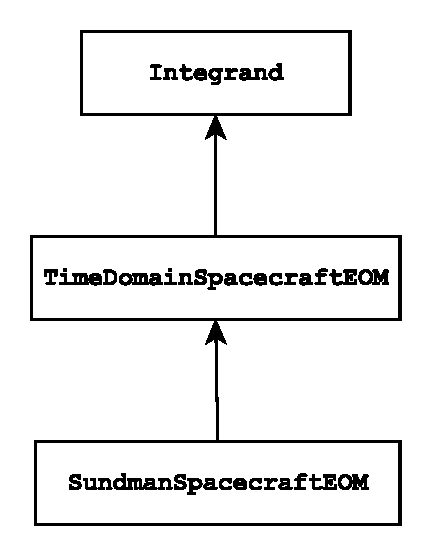
\includegraphics[width=0.3\linewidth]{./astrodynamics/Integrand_EOM_inheritance.pdf}
    \caption{\label{fig:Integrand_EOM_inheritance} Integrand inheritance diagram.}
\end{figure}

The \texttt{TimeDomainSpacecraftEOM} class encodes the first order Cartesian differential equations of motion using time as the independent variable and is derived from the \texttt{Integrand} class, which is called by implementations of the EMTG \texttt{IntegrationScheme} class. Specifically, an \texttt{IntegrationScheme} implementation calls the \texttt{TimeDomainSpacecraftEOM::evaluate} method in order to compute the current values of the differential equations (at a given epoch) as well as the orbit variational equations:

\begin{align}
\dot{\mathbf{r}} &= \mathbf{v} \label{eq:EOM_v}\\
\dot{\mathbf{v}} &= \mathbf{a} \label{eq:EOM_a} \\
\dot{m} &= -\|\mathbf{u}\|\dot{m}_{\text{max}} \label{eq:EOM_m} \\
\dot{t} &= 1 \label{eq:EOM_epoch} \\
\dot{f}_{\text{virt}} &= \dot{m}_{\text{ACS}} \label{eq:EOM_fuel} \\
\dot{o}_{\text{virt}} &= \|\mathbf{u}\|\dot{m}_{\text{max}} \label{eq:EOM_oxidizer} \\
\dot{\mathbf{\Phi}} &= \mathbf{A} \mathbf{\Phi} \label{eq:variational_eq},
\end{align}

\noindent where $\dot{m}_{\text{max}}$ is the maximum mass flow rate, $\mathbf{u} = \left[ u_x~~u_y~~uz \right]^T; \|\mathbf{u}\| \le 1$ is the maneuver control vector (\ref{subsec:TwoPointShootingLowThrustPhase}) $\mathbf{A} = \frac{\partial \dot{\mathbf{X}}}{\partial \mathbf{X}}$ is the state propagation matrix and $\mathbf{X} = \left[\mathbf{r} ~~ \mathbf{v} ~~ m ~~ t ~~ f_{\text{virt}} ~~ o_{\text{virt}} \right]^T$. Note that a differential equation is included for the current epoch $t$ (Eq. \ref{eq:EOM_epoch}), which is used to compute the current epoch if the independent variable of integration is not time (e.g. a Sundman propagator).

The \texttt{TimeDomainSpacecraftEOM::evaluate} method has two overloads, one for use with a control input, and one without (for ballistic trajectories). The \texttt{TimeDomainSpacecraftEOM::evaluate} method, first calls \texttt{TimeDomainSpacecraftEOM::computeAcceleration} (which has overloads for control/no control), which first sets the current epoch in the SpacecraftAccelerationModel and passes it pointers that it will use to extract time of flight and epoch partials from the SpacecraftAccelerationModel. Then, \texttt{TimeDomainSpacecraftEOM::computeAcceleration} calls \texttt{SpacecraftAccelerationModel::computeAcceleration}, which computes the instantaneous acceleration of the spacecraft and stores that vector. Next, \texttt{TimeDomainSpacecraftEOM::evaluate} calls \texttt{TimeDomainSpacecraftEOM::ballisticEOM}, the method that computes the first order differential equations of motion for ballistic flight. To do this, it extracts the current acceleration vector from the \texttt{SpacecraftAccelerationModel}. Despite the fact that it computes ballistic EOMs, this method also computes the differential equation for virtual chemical fuel if ACS usage is being tracked (section \ref{sec:propellant_and_dry_mass_constraints}). If the control overloaded \texttt{TimeDomainSpacecraftEOM::evaluate} is called, then \texttt{TimeDomainSpacecraftEOM::propulsionEOM} is called next, which computes the mass flow rate first order differential equations. Both overloads of \texttt{TimeDomainSpacecraftEOM::evaluate} set time derivative of current epoch (state vector entry 7) to 1.0, i.e. current epoch is (trivially) integrated, and it's time rate of change is 1.0. Finally, \texttt{TimeDomainSpacecraftEOM::evaluate} computes the variational equations by extracting the state propagation matrix from the SpacecraftAccelerationModel and computing the first order matrix differential equation.

The \texttt{SundmanDomainSpacecraftEOM} inherits from the \texttt{TimeDomainSpacecraftEOM} and applies the multiplicative transform to the t-domain EOM that transforms them to $\tau$-domain. It also computes the modified variational equations that account for this transformation:

\begin{align}
\mathring{\mathbf{X}} &= \frac{d\mathbf{X}}{d\tau} = \left( \frac{d\mathbf{X}}{dt} \right) \frac{dt}{d\tau} = \dot{\mathbf{X}}c_{\gamma} r^{\gamma} = \dot{\mathbf{X}}\eta\\
\mathring{\mathbf{\Phi}} &= \frac{\partial \mathring{\mathbf{X}}}{\partial \mathbf{X}} = \left( \frac{\partial \dot{\mathbf{X}}}{\partial \mathbf{X}}\eta + \dot{\mathbf{X}}\frac{\partial \eta}{\partial \mathbf{X}} \right) \mathbf{\Phi} = \left( \mathbf{A}\eta + \dot{\mathbf{X}}\frac{\partial \eta}{\partial \mathbf{X}} \right) \mathbf{\Phi}
\end{align}

\noindent where $\eta = c_{\gamma}r^{\gamma}$ is the multiplicative Sundman transformation function, $c_{\gamma}$ is a constant, which is set equal to the Universe length unit (LU), and $\gamma$ is the Sundman power constant, which is set to 1.0 in the current implementation. This means that the integration time steps correspond to a eccentric anomaly (to within a constant scale factor).




